% =====================================================================
% GRAPHIOT -- Presentation for supervisor meeting
% Detecting Harmful LLM-Agent Commands in Industrial IoT
% with Task-Aware Graph Neural Networks
% Beamer, English slides. Speech: speech_fr.tex (French, casual).
% No em-dash, no special symbols. Figures are TikZ (self-contained).
% =====================================================================
\documentclass[aspectratio=169]{beamer}

\usetheme{default}
\usecolortheme{owl} % falls back gracefully; see fallback below
% ---- robust fallback if owl colortheme is missing ----
\makeatletter
\@ifundefined{beamer@colorthemeowlloaded}{%
  \usecolortheme{default}%
}{}
\makeatother

\usepackage[utf8]{inputenc}
\usepackage[T1]{fontenc}
\usepackage{amsmath,amssymb}
\usepackage{tikz}
\usetikzlibrary{arrows.meta,positioning,shapes.geometric,fit,backgrounds,calc}
\usepackage{booktabs}

% ---- Colors (dark, professional) ----
\definecolor{bg}{HTML}{14181F}
\definecolor{fg}{HTML}{E8ECF2}
\definecolor{accent}{HTML}{4FA3FF}
\definecolor{accent2}{HTML}{FF9F43}
\definecolor{good}{HTML}{3FB68B}
\definecolor{bad}{HTML}{E5556E}
\definecolor{muted}{HTML}{8A94A6}
\definecolor{panel}{HTML}{1E242E}

\setbeamercolor{background canvas}{bg=bg}
\setbeamercolor{normal text}{fg=fg}
\setbeamercolor{frametitle}{fg=fg}
\setbeamercolor{title}{fg=fg}
\setbeamercolor{itemize item}{fg=accent}
\setbeamercolor{itemize subitem}{fg=accent2}
\setbeamercolor{block title}{bg=panel,fg=accent}
\setbeamercolor{block body}{bg=panel,fg=fg}
\setbeamerfont{frametitle}{size=\large,series=\bfseries}
\setbeamertemplate{navigation symbols}{}
\setbeamertemplate{itemize items}[circle]

% footline with slide number
\setbeamertemplate{footline}{%
  \hbox{\hskip0.9em\color{muted}\tiny GRAPHIOT \hfill
  \insertframenumber/\inserttotalframenumber\hskip0.9em}\vskip4pt}

\newcommand{\key}[1]{\textcolor{accent}{\textbf{#1}}}
\newcommand{\warn}[1]{\textcolor{accent2}{\textbf{#1}}}

\title{\textbf{Detecting Harmful LLM-Agent Commands in Industrial IoT}}
\subtitle{Task-Aware Graph Neural Networks}
\author{Billal Mokhtari \and Yulliwas Ameur \and Samia Bouzefrane}
\institute{CEDRIC Laboratory, Cnam Paris \\ BATTwin project}
\date{October 2026}

\begin{document}

% =====================================================================
% SLIDE 1 -- Title
% =====================================================================
{\setbeamertemplate{footline}{}
\begin{frame}
  \titlepage
  \begin{center}
  \footnotesize\textcolor{muted}{IEEE Internet of Things Journal, Special Issue on
  Graph Representation Learning for IoT}
  \end{center}
\end{frame}}

% =====================================================================
% SLIDE 2 -- What is happening (context)
% =====================================================================
\begin{frame}{The new situation: LLM agents are driving factories}
\begin{columns}[T]
\begin{column}{0.56\textwidth}
\begin{itemize}
  \item An \key{LLM agent} now assists the human operator of a plant.
  \item It cannot touch the machines directly. It acts through an
        \key{edge gateway} that offers a few tools.
  \item The gateway turns each tool call into a \key{Modbus write} to a PLC.
  \item The agent works with the rights of a \key{trusted operator}.
\end{itemize}
\vspace{0.4em}
\begin{block}{The problem in one line}
A misled or hijacked agent can send a command that is \warn{valid,
authorized and on the allow-list}, yet still harmful.
\end{block}
\end{column}
\begin{column}{0.44\textwidth}
\centering
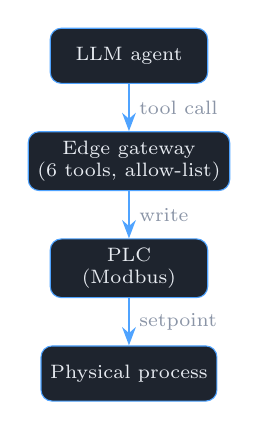
\begin{tikzpicture}[font=\scriptsize,node distance=6mm,
   box/.style={draw=accent,fill=panel,rounded corners,text=fg,
   minimum width=20mm,minimum height=7mm,align=center}]
  \node[box] (agent) {LLM agent};
  \node[box,below=of agent] (gw) {Edge gateway\\(6 tools, allow-list)};
  \node[box,below=of gw] (plc) {PLC\\(Modbus)};
  \node[box,below=of plc] (proc) {Physical process};
  \draw[-{Stealth},accent,thick] (agent)--node[right,text=muted]{tool call}(gw);
  \draw[-{Stealth},accent,thick] (gw)--node[right,text=muted]{write}(plc);
  \draw[-{Stealth},accent,thick] (plc)--node[right,text=muted]{setpoint}(proc);
\end{tikzpicture}
\end{column}
\end{columns}
\end{frame}

% =====================================================================
% SLIDE 3 -- The dangerous command (intuition)
% =====================================================================
\begin{frame}{The hardest command to catch: context-shifted}
\begin{columns}[T]
\begin{column}{0.5\textwidth}
\textbf{Everyday analogy.}\\[0.3em]
``Drive at 90 km/h'' is:
\begin{itemize}
  \item fine on the \textcolor{good}{motorway},
  \item dangerous in front of a \textcolor{bad}{school}.
\end{itemize}
\vspace{0.6em}
Same command. Only the \key{situation} changed.
\end{column}
\begin{column}{0.5\textwidth}
\textbf{In the plant.}\\[0.3em]
Write \texttt{coating\_speed = 2.40 m/min}:
\begin{itemize}
  \item \textcolor{good}{steady state}: dryer hot, coating dries, good batch;
  \item \textcolor{bad}{dryer warm-up}: oven still cold, the film comes out
        wet, the batch is ruined.
\end{itemize}
\end{column}
\end{columns}
\vspace{0.6em}
\begin{center}
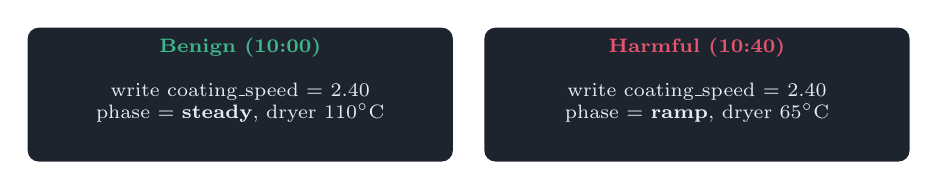
\begin{tikzpicture}[font=\scriptsize]
  \fill[panel,rounded corners] (-5.6,-0.9) rectangle (-0.2,0.8);
  \fill[panel,rounded corners] (0.2,-0.9) rectangle (5.6,0.8);
  \node[text=good] at (-2.9,0.55) {\textbf{Benign (10:00)}};
  \node[text=fg,align=center] at (-2.9,-0.15)
    {write coating\_speed = 2.40\\ phase = \textbf{steady}, dryer 110$^\circ$C};
  \node[text=bad] at (2.9,0.55) {\textbf{Harmful (10:40)}};
  \node[text=fg,align=center] at (2.9,-0.15)
    {write coating\_speed = 2.40\\ phase = \textbf{ramp}, dryer 65$^\circ$C};
\end{tikzpicture}
\end{center}
\end{frame}

% =====================================================================
% SLIDE 4 -- Why single-view defenses fail
% =====================================================================
\begin{frame}{Why every current defense is blind to it}
\begin{center}
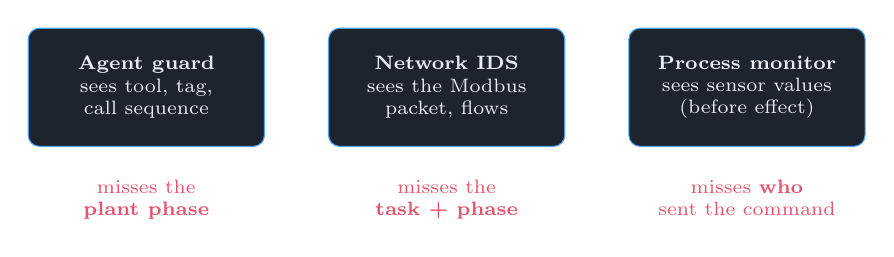
\begin{tikzpicture}[font=\scriptsize,
   v/.style={draw,fill=panel,rounded corners,text=fg,align=center,
   minimum width=30mm,minimum height=15mm}]
  \node[v,draw=accent] (ag) {\textbf{Agent guard}\\ sees tool, tag,\\ call sequence};
  \node[v,draw=accent,right=8mm of ag] (net) {\textbf{Network IDS}\\ sees the Modbus\\ packet, flows};
  \node[v,draw=accent,right=8mm of net] (pr) {\textbf{Process monitor}\\ sees sensor values\\ (before effect)};
  \node[text=bad,below=3mm of ag,align=center] (a2){misses the\\ \textbf{plant phase}};
  \node[text=bad,below=3mm of net,align=center] (n2){misses the\\ \textbf{task + phase}};
  \node[text=bad,below=3mm of pr,align=center] (p2){misses \textbf{who}\\ sent the command};
\end{tikzpicture}
\end{center}
\vspace{0.3em}
\begin{block}{Observation 1 (single-view blindness)}
If a score depends on a command only through its triple
$(a,\kappa,\mathrm{bin}(v))$ and agent history, then the benign command and
its harmful twin get the \warn{exact same score}. Same for a network view, and
for a process view before the effect appears.
\end{block}
\end{frame}

% =====================================================================
% SLIDE 5 -- Formal definition (equations)
% =====================================================================
\begin{frame}{Defining the command and the slice}
A command is a 4-tuple:
\begin{equation*}
  c = (a,\ \kappa,\ v,\ t)
  \qquad\text{\scriptsize tool, target tag, value, time}
\end{equation*}
\vspace{-0.3em}
\begin{itemize}
  \item $\mathrm{bin}(v)$ maps the value to one of \key{$Q$ quantile bins}
        learned on benign data.
  \item $\mathcal{C}_{\text{benign}}$ = set of triples
        $(a,\kappa,\mathrm{bin}(v))$ ever seen in benign training.
\end{itemize}
\vspace{0.3em}
\begin{block}{Definition: context-shifted command}
$c$ is context-shifted if all three hold:
\[
\underbrace{(a,\kappa,\mathrm{bin}(v))\in\mathcal{C}_{\text{benign}}}_{\text{looks normal}}
\;\wedge\;
\underbrace{\text{allow-list permits it}}_{\text{passes the gateway}}
\;\wedge\;
\underbrace{\text{oracle} = \text{harmful}}_{\text{actually damages}}
\]
\end{block}
\centering\footnotesize\textcolor{muted}{This is the exact test slice we report separately.}
\end{frame}

% =====================================================================
% SLIDE 6 -- The idea: one graph at the gateway
% =====================================================================
\begin{frame}{Our idea: link everything in one graph at the gateway}
\begin{columns}[T]
\begin{column}{0.46\textwidth}
\begin{itemize}
  \item Build a \key{dynamic heterogeneous graph} from the gateway logs and the
        fieldbus.
  \item It connects the \key{task} to the \key{plant state}, which no single
        view does.
  \item A temporal GNN learns, from \key{benign data only}, how likely each
        command is in its context.
  \item Score each command \key{before} its effect appears.
\end{itemize}
\end{column}
\begin{column}{0.54\textwidth}
\centering
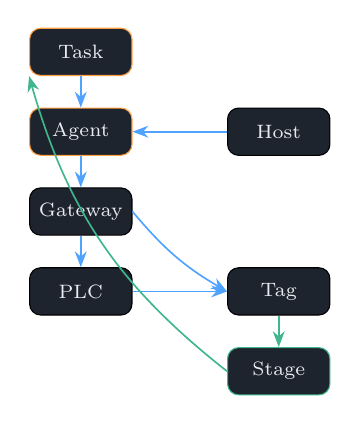
\begin{tikzpicture}[font=\scriptsize,node distance=4mm,
   n/.style={draw,fill=panel,rounded corners,text=fg,align=center,
   minimum height=6mm,minimum width=13mm},
   e/.style={-{Stealth},accent,semithick}]
  \node[n,draw=accent2] (task) {Task};
  \node[n,draw=accent2,below=of task] (agent) {Agent};
  \node[n,below=of agent] (gw) {Gateway};
  \node[n,right=12mm of agent] (host) {Host};
  \node[n,below=of gw] (plc) {PLC};
  \node[n,right=12mm of plc] (tag) {Tag};
  \node[n,draw=good,below=of tag] (stage) {Stage};
  \draw[e] (task)--(agent);
  \draw[e] (agent)--(gw);
  \draw[e] (host)--(agent);
  \draw[e] (gw)--(plc);
  \draw[e] (plc)--(tag);
  \draw[e] (gw.east)to[bend right=10](tag.west);
  \draw[e,good] (tag)--(stage);
  \draw[e,good] (stage.west)to[bend left=18]node[below,text=muted,pos=0.5]{}(task.south west);
\end{tikzpicture}
\\[0.3em]
\footnotesize\textcolor{muted}{Task and Stage are the nodes that single-view
detectors never connect.}
\end{column}
\end{columns}
\end{frame}

% =====================================================================
% SLIDE 7 -- Graph schema
% =====================================================================
\begin{frame}{The task--plant graph (schema)}
\footnotesize
\begin{columns}[T]
\begin{column}{0.5\textwidth}
\textbf{Node types}
\begin{tabular}{@{}ll@{}}
\toprule
Node & Key features \\
\midrule
Task  & type, target stage, tag set \\
Agent & session age, call rate \\
Gateway & call rate, error rate \\
Host & role, flow stats \\
PLC & request rate \\
Tag & value, rolling mean/std \\
Stage & phase, time in phase \\
\bottomrule
\end{tabular}
\end{column}
\begin{column}{0.5\textwidth}
\textbf{Edge types}
\begin{tabular}{@{}ll@{}}
\toprule
Edge & Carries \\
\midrule
assigned & time since assign. \\
invokes & tool id \\
writes/reads & FC, value, delta \\
flow & NetFlow features \\
controls, belongs & static \\
\bottomrule
\end{tabular}
\vspace{0.6em}
\begin{block}{Strict rule}
No feature contains a \warn{recipe}, an \warn{operating limit} or a
\warn{twin output}. The detector never sees them.
\end{block}
\end{column}
\end{columns}
\vspace{0.3em}
\centering\textcolor{muted}{Snapshots over windows $\Delta=10$ s, stride $5$ s.}
\end{frame}

% =====================================================================
% SLIDE 8 -- The model pipeline (equations part 1)
% =====================================================================
\begin{frame}{The model: from graph to probability}
\begin{center}
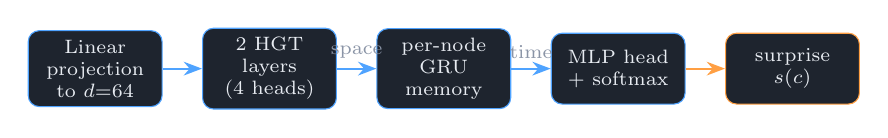
\begin{tikzpicture}[font=\scriptsize,node distance=5mm,
   s/.style={draw=accent,fill=panel,rounded corners,text=fg,align=center,
   minimum height=9mm,minimum width=17mm}]
  \node[s] (proj) {Linear\\ projection\\ to $d{=}64$};
  \node[s,right=of proj] (hgt) {2 HGT\\ layers\\ (4 heads)};
  \node[s,right=of hgt] (gru) {per-node\\ GRU\\ memory};
  \node[s,right=of gru] (head) {MLP head\\ + softmax};
  \node[s,draw=accent2,right=of head] (score) {surprise\\ $s(c)$};
  \draw[-{Stealth},accent,thick] (proj)--(hgt);
  \draw[-{Stealth},accent,thick] (hgt)--node[above,text=muted]{space}(gru);
  \draw[-{Stealth},accent,thick] (gru)--node[above,text=muted]{time}(head);
  \draw[-{Stealth},accent2,thick] (head)--(score);
\end{tikzpicture}
\end{center}
\vspace{0.2em}
Memory carries information across snapshots:
\begin{equation*}
  \mathbf{m}_v^{\,t} = \mathrm{GRU}\!\left(\mathbf{h}_v^{\,t},\ \mathbf{m}_v^{\,t-1}\right)
\end{equation*}
\begin{itemize}
  \item HGT mixes information \key{across the graph} (neighbours, typed edges).
  \item GRU mixes information \key{across time} (recent history of each node).
  \item A new node starts from a zero memory.
\end{itemize}
\end{frame}

% =====================================================================
% SLIDE 9 -- Likelihood and score (equations part 2)
% =====================================================================
\begin{frame}{Task-conditioned likelihood and the score}
Trained on benign data only, the model predicts the written tag and value bin
from the context just before the command:
\begin{equation*}
  p_\theta\!\left(\kappa,\ \mathrm{bin}(v)\ \middle|\
  \mathbf{m}_{\tau}^{\,t^-},\
  \mathbf{m}_{\text{agent}}^{\,t^-},\
  \mathbf{m}_{\text{stage}(\kappa)}^{\,t^-},\
  \mathbf{m}_{\kappa}^{\,t^-}\right)
\end{equation*}
\centering\footnotesize\textcolor{muted}{$t^-$ = last snapshot before $t$, so the effect is never visible.}
\\[0.6em]
\flushleft
The anomaly score is the \key{surprise}:
\begin{equation*}
  s(c) = -\log p_\theta\!\left(\kappa,\ \mathrm{bin}(v)\mid\cdot\right)
\end{equation*}
\begin{itemize}
  \item A context-shifted command has a \key{frequent triple} but an
        \key{unlikely context}, so $s(c)$ is high only if the model truly uses
        the task and the stage.
  \item Alarm threshold set on benign validation at a \key{1\% false positive rate}.
\end{itemize}
\end{frame}

% =====================================================================
% SLIDE 10 -- Evaluation protocol (no results)
% =====================================================================
\begin{frame}{How we test it honestly (a test that can fail)}
\begin{columns}[T]
\begin{column}{0.5\textwidth}
\textbf{Independent attacks}
\begin{itemize}
  \item A \key{red-team LLM} from a different family generates the attacks.
  \item It gets only a MITRE ATT\&CK for ICS technique + the plant docs.
  \item No hand-written attack script.
\end{itemize}
\vspace{0.4em}
\textbf{External oracle}
\begin{itemize}
  \item Labels by checking \key{process outputs} against operating limits.
  \item The detector \warn{never sees} these limits.
\end{itemize}
\end{column}
\begin{column}{0.5\textwidth}
\textbf{Baselines}
\begin{itemize}
  \item B0 phase-aware value table
  \item B1 allow-list
  \item B2 same-feature tabular (XGBoost)
  \item B3 network view (E-GraphSAGE)
  \item B4 agent view (AIRGuard)
  \item B5 LLM judge
\end{itemize}
\vspace{0.3em}
\textbf{Splits:} chronological (70/10/20), never random. Thresholds never see
red-team data.
\end{column}
\end{columns}
\end{frame}

% =====================================================================
% SLIDE 11 -- Adaptive attacker (equation)
% =====================================================================
\begin{frame}{The strongest test: an adaptive, effect-preserving attacker}
A grey-box attacker tries to stay harmful while lowering our score:
\begin{equation*}
  \min_{\delta\in\mathcal{R}_B(e)}\ \max_{c\in e\oplus\delta}\ s_\theta(c)
  \qquad\text{s.t.}\qquad
  \mathrm{Oracle}(e\oplus\delta) = \text{harmful}
\end{equation*}
\begin{itemize}
  \item $e$ is an episode, $\mathcal{R}_B(e)$ the \key{realizable edits} with at
        most $B$ added events.
  \item Allowed edits: insert benign reads, interleave old benign commands,
        split a change, shift in time.
  \item Every edit must \warn{keep the physical effect} (checked by the oracle).
  \item Budgets $B \in \{0,4,8\}$.
\end{itemize}
\vspace{0.3em}
\centering\footnotesize\textcolor{muted}{This stops us from claiming robustness we do not have.}
\end{frame}

% =====================================================================
% SLIDE 12 -- Pre-registered hypotheses (not results)
% =====================================================================
\begin{frame}{Pre-registered hypotheses (they are allowed to fail)}
\begin{block}{H1 (main)}
On context-shifted commands, our recall at 1\% FPR beats B0, B2, B3, B4, B5 by
at least 10 points (McNemar, Holm-corrected $p<0.05$).
\end{block}
\begin{block}{H2 (where the signal comes from)}
Single-view ablations stay at AUROC $\le 0.6$; removing the \key{task} node
hurts more than removing the network subgraph.
\end{block}
\begin{block}{H3 (robustness)}
At $B=4$, fewer harmful episodes evade our model than B2 and B4.
\end{block}
\vspace{0.2em}
\centering\footnotesize\textcolor{muted}{If H1 fails against B0, the task adds nothing beyond phase statistics. We report that too.}
\end{frame}

% =====================================================================
% SLIDE 13 -- THINGS TO CHANGE IN THE ARTICLE (flag slide 1)
% =====================================================================
\begin{frame}{\warn{To fix in the article} (1/2): notation and timeline}
\textbf{Notation clash}
\begin{itemize}
  \item $\tau$ is used for \key{two different things}: the task (Sec. IV,
        $\mathbf{m}_\tau$) and the oracle margin (``leaves its limits by at least
        $\tau$'', Sec. V). \warn{Rename one}, e.g. margin $\to \varepsilon$.
\end{itemize}
\vspace{0.4em}
\textbf{Timeline is now behind}
\begin{itemize}
  \item Fallback-oracle decision was dated \warn{17/10}, OSF registration
        \warn{22/10}, pilot \warn{25/10}. We are past these.
  \item Decide the new realistic dates before submission (deadline 30/11).
\end{itemize}
\end{frame}

% =====================================================================
% SLIDE 14 -- THINGS TO CHANGE IN THE ARTICLE (flag slide 2)
% =====================================================================
\begin{frame}{\warn{To fix in the article} (2/2): content decisions}
\begin{itemize}
  \item \textbf{Placeholders to fill:} the abstract result sentence, all
        $[X]$ in the tables, model names and sizes (operator and red-team),
        benign hours and command counts.
  \item \textbf{Final hyperparameters + search grid} (at most 2 values each,
        chosen on benign validation only), training time, parameter count.
  \item \textbf{Oracle choice} (primary twin replay vs fallback) must be
        locked, with the limits table in the supplement.
  \item \textbf{H2 claim ``AUROC $\le 0.6$''} is strong. Confirm it survives the
        pilot, or soften it.
  \item \textbf{Figure 1} (architecture) is still a placeholder box: produce the
        final vector PDF.
  \item \textbf{Scope sentence:} double-check the ``emulated vs synthetic''
        wording is consistent with the dataset paper.
\end{itemize}
\end{frame}

% =====================================================================
% SLIDE 15 -- Next steps / conclusion
% =====================================================================
\begin{frame}{Where we stand and what is next}
\begin{columns}[T]
\begin{column}{0.56\textwidth}
\textbf{The contribution}
\begin{itemize}
  \item A named, measurable class: \key{context-shifted commands}.
  \item A \key{task-conditioned likelihood} at the edge, trained on benign data.
  \item A test that can fail: independent red-team + external oracle +
        adaptive attacker.
\end{itemize}
\end{column}
\begin{column}{0.44\textwidth}
\textbf{Next steps}
\begin{itemize}
  \item Lock the oracle and the dates.
  \item Run the pilot and the go/no-go test.
  \item Run the main campaign.
  \item Fill the tables and the final figure.
\end{itemize}
\end{column}
\end{columns}
\vspace{0.8em}
\begin{center}
\large\textcolor{accent}{Thank you. Questions and feedback welcome.}
\end{center}
\end{frame}

\end{document}
